\documentclass[aspectratio=169, 10pt]{beamer}

% Formal IEEE-style presentation theme with beautiful rounded shadows
\usetheme{Boadilla}
\usecolortheme{seahorse}
\usefonttheme{professionalfonts}

\usepackage{graphicx}
\usepackage{booktabs}
\usepackage{multirow}
\usepackage{tikz} 
\usepackage{pifont} % Added for checkmarks and crosses
\usepackage{amsmath}

% Enhancing visual appeal of lists and blocks
\setbeamertemplate{navigation symbols}{}
\setbeamertemplate{itemize item}{\color{blue!70!black}$\blacktriangleright$} 
\setbeamertemplate{itemize subitem}{\color{teal}$\bullet$}
\setbeamertemplate{caption}[numbered]
\setbeamertemplate{bibliography item}[text]
\setbeamertemplate{blocks}[rounded][shadow=true] 

% ==========================================
% HEADER LOGO CONFIGURATION
% ==========================================
\addtobeamertemplate{frametitle}{}{%
\begin{tikzpicture}[remember picture,overlay]
\node[anchor=north east, yshift=-0.1cm, xshift=-0.2cm] at (current page.north east) {%
    \IfFileExists{faculty_of_engineering.jpeg}{
\includegraphics[height=1.5cm]{faculty_of_engineering.jpeg}}{}%
};
\end{tikzpicture}}

% ==========================================
% BULLETPROOF CUSTOM FOOTER
% ==========================================
\makeatletter
\setbeamertemplate{footline}{
  \leavevmode%
  \hbox{%
  \begin{beamercolorbox}[wd=.33\paperwidth,ht=2.5ex,dp=1.125ex,center]{author in head/foot}%
    \usebeamerfont{author in head/foot}\textbf{\insertshortauthor}
  \end{beamercolorbox}%
  \begin{beamercolorbox}[wd=.38\paperwidth,ht=2.5ex,dp=1.125ex,center]{title in head/foot}%
    \usebeamerfont{title in head/foot}\textbf{Reference-Guided Few-Shot Segmentation with Foundation Models, 2026}
  \end{beamercolorbox}%
  \begin{beamercolorbox}[wd=.29\paperwidth,ht=2.5ex,dp=1.125ex,right]{date in head/foot}%
    \usebeamerfont{date in head/foot}\textbf{Page \insertframenumber{} of \inserttotalframenumber}\hspace*{2ex}
  \end{beamercolorbox}}%
  \vskip0pt%
}
\makeatother

\title[Few-Shot Image Segmentation]{Reference-Guided Few-Shot Segmentation with Foundation Models}
\subtitle{PhD Research Proposal}
\author[Omar Ahmed Fouad Hassan Wasfy]{Omar Ahmed Fouad Hassan Wasfy}
\institute[Alexandria University]{
Computer and Systems Engineering Department, Faculty of Engineering\\
 Alexandria University \\
 \vspace{1cm}
 \textbf{Supervisors: Prof. Dr. Mohamed Ismail and Prof. Dr. Nagia Ghanem}
 \\
 \vspace{0.5cm}
 \textbf{2026}
}
\date{} 

\begin{document}

% Slide 1
\begin{frame}
    \titlepage
\end{frame}

% Slide 2
\begin{frame}{Outline}
 \tableofcontents[hideallsubsections]
\end{frame}


% ==========================================
% SECTION 1: INTRODUCTION & BACKGROUND
% ==========================================
\section{Introduction \& Background}

% Slide 3
\begin{frame}{Top-Tier Venues Referenced in This Presentation}
\begin{columns}[T]
    \begin{column}{0.48\textwidth}
        \begin{block}{Computer Vision}
            \begin{itemize}
                \item \textbf{CVPR} \\ \small IEEE/CVF Conference on Computer Vision and Pattern Recognition
                \item \textbf{ICCV} \\ \small IEEE/CVF International Conference on Computer Vision
                \item \textbf{IJCV} \\ \small International Journal of Computer Vision
                \item \textbf{TPAMI} \\ \small IEEE Transactions on Pattern Analysis and Machine Intelligence
            \end{itemize}
        \end{block}
    \end{column}

    \begin{column}{0.48\textwidth}
        \begin{block}{Machine Learning / AI / Medical}
            \begin{itemize}
                \item \textbf{ICLR} \\ \small International Conference on Learning Representations
                \item \textbf{NeurIPS} \\ \small Conference on Neural Information Processing Systems
                \item \textbf{AAAI} \\ \small AAAI Conference on Artificial Intelligence
                \item \textbf{MICCAI} \\ \small Medical Image Computing and Computer Assisted Intervention
            \end{itemize}
        \end{block}
    \end{column}
\end{columns}

\vspace{0.3cm}
\centering
\footnotesize The listed venues comprise top-tier (A*) conferences and high-impact journals in Computer Vision, Machine Learning, and Medical Imaging.
\end{frame}

% Slide 4
\begin{frame}{From Closed-Set \& Zero-Shot to Few-Shot Segmentation}
    \begin{columns}[T]
        \begin{column}{0.32\textwidth}
            \begin{alertblock}{Closed-Set Segmentation}
                \begin{itemize}
                    \item Trained on a \textbf{fixed, predefined} label space.
                    \item Requires \textbf{large-scale pixel-level annotations}.
                    \item \textbf{Limited generalization} to unseen object classes.
                \end{itemize}
            \end{alertblock}
        \end{column}

        \begin{column}{0.32\textwidth}
            \begin{block}{Zero-Shot Segmentation}
                \begin{itemize}
                    \item Transfers knowledge via \textbf{semantic priors} (e.g., \textit{text prompts}).
                    \item Utilizes \textbf{geometric prompts} (e.g., points, boxes).
                    \item Requires \textbf{no task-specific annotations}.
                    \item \textbf{Weak spatial precision} (coarse masks).
                \end{itemize}
            \end{block}
        \end{column}
        
        \begin{column}{0.32\textwidth}
            \begin{exampleblock}{Few-Shot Segmentation}
                \begin{itemize}
                    \item Adapts using \textbf{few labeled examples} (1--5 images) \cite{shaban2017one}.
                    \item Learns \textbf{class-specific representations} from support data.
                    \item \textbf{Accurate pixel-level localization}.
                    \item \textbf{Middle Ground:} balances generalization and supervision.
                \end{itemize}
            \end{exampleblock}
        \end{column}
    \end{columns}
\end{frame}

% Slide 5
\begin{frame}{Vision Foundation Models \& Visual Prompting}
    \begin{columns}[T]
        \begin{column}{0.48\textwidth}
            \begin{block}{Self-Supervised Learning at Scale}
                \begin{itemize}
                    \item Models trained on unprecedented scales of unannotated images (e.g., DINOv2) \cite{oquab2023dinov2}.
                    \item Discards traditional convolutions for long-range multi-head self-attention.
                    \item Yields highly robust feature embeddings with dense, part-level semantic understanding.
                \end{itemize}
            \end{block}
        \end{column}
        
        \begin{column}{0.48\textwidth}
            \begin{exampleblock}{Visual Conditioning (Prompting)}
                \begin{itemize}
                    \item \textbf{The Paradigm Shift:} Appends learnable tokens to input features while keeping massive foundation backbone weights \textbf{strictly frozen}.
                    \item Preserves generalized representation capacity.
                    \item Minimizes the risk of overfitting during adaptation where data is scarce.
                \end{itemize}
            \end{exampleblock}
        \end{column}
    \end{columns}
\end{frame}


% Slide 6
\begin{frame}{Reference-Guided Few-Shot Segmentation \& System Setup}
    \begin{block}{Task Definition: Open-Set Generalization}
        A conditional dense prediction task aiming to delineate a target object in a query image, guided strictly by a small set of annotated reference examples. It operates \textbf{class-agnostic}, relying entirely on visual patterns rather than predefined text labels.
    \end{block}

    \begin{columns}[T]
        \begin{column}{0.48\textwidth}
            \textbf{Inputs}
            \begin{itemize}
                \item \textbf{Support Set (Reference Set):} A few images pairing the target object with a pixel-level spatial mask.
                \item \textbf{Query Image (Target Image):} Unlabeled target environment containing complex scenes and novel conditions.
            \end{itemize}
        \end{column}
        \begin{column}{0.48\textwidth}
            \textbf{Outputs \& Optimization}
            \begin{itemize}
                \item \textbf{Output:} A continuous probability map thresholded into a discrete binary mask.
                \item \textbf{Optimization:} A weighted dual-objective combination of Binary Cross-Entropy Loss and structural Dice Loss.
            \end{itemize}
        \end{column}
    \end{columns}
\end{frame}

% Slide 7
\begin{frame}{Core Technical Challenges}
    Adapting generic foundation models to Few-Shot Segmentation introduces severe mathematical bottlenecks:
    
    \begin{alertblock}{The Adaptation Challenges}
        \begin{itemize}
            \item \textbf{Cross-Image Correspondence:} Establishing associations despite radical differences in camera viewpoint, object pose, and lighting.
            \item \textbf{Appearance Variability:} Handling massive intra-class variation, scale changes, elastic deformation, and partial occlusion.
            \item \textbf{Distractor Suppression:} Distinguishing the target from visually similar elements densely clustered in complex environments.
            \item \textbf{Prompt Sensitivity:} Ensuring stability when automatically generated geometric prompts are placed suboptimally on object boundaries.
        \end{itemize}
    \end{alertblock}
\end{frame}



% Slide 8
\begin{frame}{The Segment Anything Model (SAM) \textbf{(ICCV 2023)}}
    % Top Section: Technical Description
    \begin{block}{Architecture \cite{kirillov2023segment}}
        \begin{itemize}
            \item \textbf{Image Encoder:} Masked Autoencoder (MAE) pre-trained Vision Transformer (ViT) generating high-dimensional image embeddings.
            \item \textbf{Prompt Encoder:} Positional encodings for points/boxes and convolutional layers for dense masks.
            \item \textbf{Mask Decoder:} Lightweight two-way transformer mapping image and prompt embeddings to valid segmentation masks.
        \end{itemize}
    \end{block}

    \vfill 

    % Bottom Section: Full-Width Visualization
    \centering
    \IfFileExists{SAM.png}{
        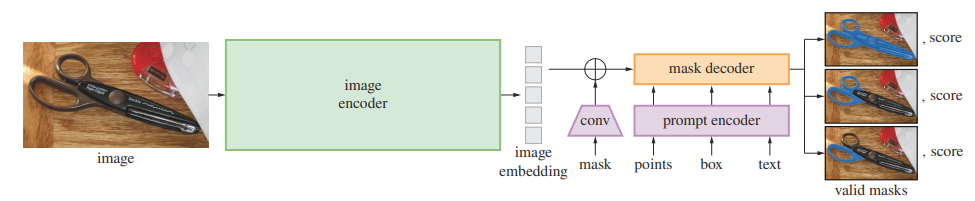
\includegraphics[width=\textwidth, height=0.45\textheight, keepaspectratio]{SAM.png}
    }{
        \begin{tikzpicture}
            \draw[dashed] (0,0) rectangle (\textwidth, 3) node[pos=.5] {Placeholder: SAM.png (Full Width)};
        \end{tikzpicture}
    }
\end{frame}

% Slide 9
\begin{frame}{The Semantic-Geometric Gap}
    \begin{block}{The Limitation of Scale (SA-1B Dataset)}
        SAM is trained on 1 billion high-quality masks, enforcing extreme geometric robustness. However, these masks are purely structural; they contain \textbf{no class or category labels}.
    \end{block}

    \begin{alertblock}{The Semantic Deficit}
        \begin{itemize}
            \item SAM learns \textit{"what constitutes an object"} but never learns \textit{"what the object is"}.
            \item It cannot natively process a support image-mask pair to locate a semantically identical object in a query image.
            \item External conditioning mechanisms must be engineered to translate semantic intent into SAM's native geometric prompt language.
        \end{itemize}
    \end{alertblock}
\end{frame}

% ==========================================
% SECTION 4: ENHANCED METHODOLOGIES
% ==========================================
\section{Methodological Taxonomies}

% Slide 10
\begin{frame}{Taxonomy of SAM-based Adaptation Strategies}
    \begin{table}[htbp]
    \centering
    \caption{Classification of Representative Few-Shot SAM Adaptation Methods}
    \renewcommand{\arraystretch}{1.05}
    \small
    \begin{tabular}{l p{0.55\linewidth}}
    \toprule
    \textbf{Paper} & \textbf{Adaptation Strategy} \\
    \midrule
    VRP-SAM (CVPR 2024) \cite{sun2024vrp} & Prompt-based adaptation (Automation) \\
    ProSAM (ICCV 2025) \cite{wang2025prosam} & Prompt-based (Probabilistic prompting) \\
    Matcher (IJCV 2025 / ICLR 2024) \cite{liu2023matcher} & Feature matching (Dense alignment) \\
    DC-SAM (TPAMI 2025) \cite{qi2025dcsam} & Consistency-based (Cyclic validation) \\
    Bridge the Points (NeurIPS 2024) \cite{zhang2024bridge} & Graph-based reasoning (Relational) \\
    FCP-SAM (AAAI 2025) \cite{park2025fcpsam} & Prototype-based modeling (Averaging) \\
    PerSAM (ICLR 2024) \cite{zhang2024persam} & Personalized adaptation (One-shot PEFT) \\
    DAPSAM (MICCAI 2024)\footnote{\tiny DAPSAM focuses on single-source domain generalization (SDG) rather than typical FSS; it is included here as it generates task-specific prompts and adapts the SAM foundation model to the medical domain.} \cite{wei2024prompting} & Domain-adaptive prompting (Medical SDG) \\
    \bottomrule
    \end{tabular}
    \end{table}
\end{frame}

% --- VRP-SAM ---
% Slide 11
\begin{frame}{VRP-SAM: Prompt-Based Adaptation \textbf{(CVPR 2024)}}
\textit{VRP-SAM: SAM with visual reference prompt.}
    \begin{columns}[T]
        \begin{column}{0.48\textwidth}
            \begin{block}{Motivation \& Concept \cite{sun2024vrp}}
                SAM relies on manual prompts. VRP-SAM automates this by extracting features via an auxiliary semantic encoder (ResNet) and generating compatible point embeddings via multi-head cross-attention.
            \end{block}
        \end{column}
        
        \begin{column}{0.48\textwidth}
            \begin{exampleblock}{Strengths}
                \begin{itemize}
                    \item[\textcolor{green!70!black}{\ding{51}}] Highly efficient baseline for real-time video applications.
                    \item[\textcolor{green!70!black}{\ding{51}}] Perfectly preserves SAM's native geometric boundary precision.
                \end{itemize}
            \end{exampleblock}
            \begin{alertblock}{Limitations}
                \begin{itemize}
                    \item[\textcolor{red}{\ding{55}}] Highly susceptible to prompt sensitivity.
                    \item[\textcolor{red}{\ding{55}}] Rigid prompts fail if the target undergoes severe structural deformation.
                \end{itemize}
            \end{alertblock}
        \end{column}
    \end{columns}
\end{frame}

% Slide 12
\begin{frame}{VRP-SAM: Architecture \textbf{(CVPR 2024)}}
    \begin{center}
        \IfFileExists{VRP-SAM-3.png}{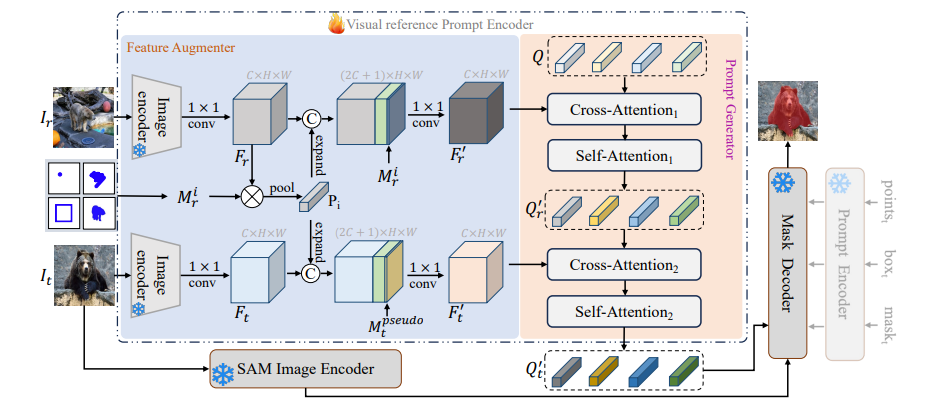
\includegraphics[width=\textwidth, height=0.85\textheight, keepaspectratio]{VRP-SAM-3.png}}{\textbf{[Placeholder: VRP-SAM-3.png]}}
    \end{center}
\end{frame}

% --- PROSAM ---
% Slide 13
\begin{frame}{ProSAM: Probabilistic Prompting \textbf{(ICCV 2025)}}
\textit{ProSAM: Enhancing the robustness of SAM-based visual reference segmentation with probabilistic prompts.}
    \begin{columns}[T]
        \begin{column}{0.48\textwidth}
            \begin{block}{Motivation \& Concept \cite{wang2025prosam}}
                Deterministic prompts are brittle. ProSAM models the prompt space as a continuous multivariate distribution. A Laplacian penalty physically pushes expected prompts toward flat, central regions of the target.
            \end{block}
        \end{column}
        
        \begin{column}{0.48\textwidth}
            \begin{exampleblock}{Strengths}
                \begin{itemize}
                    \item[\textcolor{green!70!black}{\ding{51}}] Exceptionally robust to boundary ambiguities.
                    \item[\textcolor{green!70!black}{\ding{51}}] Marginalizes uncertainty via Monte Carlo sampling.
                \end{itemize}
            \end{exampleblock}
            \begin{alertblock}{Limitations}
                \begin{itemize}
                    \item[\textcolor{red}{\ding{55}}] Processing multiple sampled prompts sequentially massively increases latency.
                    \item[\textcolor{red}{\ding{55}}] Unsuitable for high-speed tracking.
                \end{itemize}
            \end{alertblock}
        \end{column}
    \end{columns}
\end{frame}

% Slide 14
\begin{frame}{ProSAM: Architecture \textbf{(ICCV 2025)}}
    \begin{center}
        \IfFileExists{PRO-SAM-3.png}{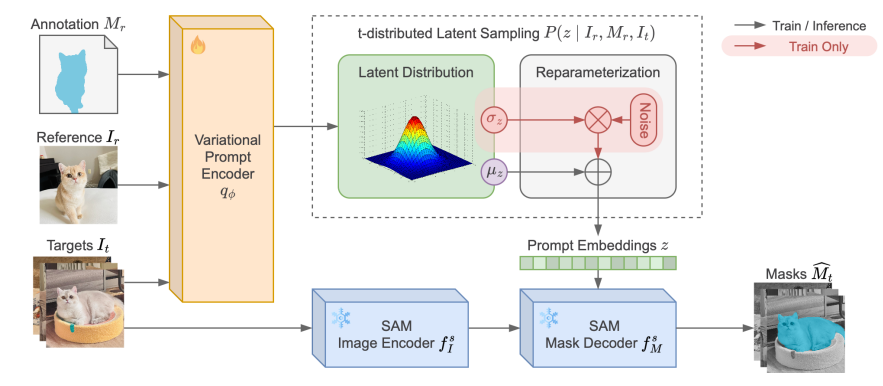
\includegraphics[width=\textwidth, height=0.85\textheight, keepaspectratio]{PRO-SAM-3.png}}{\textbf{[Placeholder: PRO-SAM-3.png]}}
    \end{center}
\end{frame}

% --- MATCHER ---
% Slide 15
\begin{frame}{Matcher: Feature Matching Approach \textbf{(IJCV 2025 \& ICLR 2024)}}
\textit{Matcher: Segment anything with one shot using all-purpose feature matching.}
    \begin{columns}[T]
        \begin{column}{0.48\textwidth}
            \begin{block}{Motivation \& Concept \cite{liu2023matcher}}
                Bypasses prompt training entirely. Constructs dense correlation volumes using DINOv2 self-supervised features and enforces forward/reverse cycle-consistency to eliminate mathematical outliers.
            \end{block}
        \end{column}
        
        \begin{column}{0.48\textwidth}
            \begin{exampleblock}{Strengths}
                \begin{itemize}
                    \item[\textcolor{green!70!black}{\ding{51}}] Elegant, tuning-free zero-shot operation.
                    \item[\textcolor{green!70!black}{\ding{51}}] Requires absolutely zero task-specific meta-training.
                \end{itemize}
            \end{exampleblock}
            \begin{alertblock}{Limitations}
                \begin{itemize}
                    \item[\textcolor{red}{\ding{55}}] Highly prone to distractor suppression failures. 
                    \item[\textcolor{red}{\ding{55}}] Visually similar background elements inevitably trigger false-positive matches.
                \end{itemize}
            \end{alertblock}
        \end{column}
    \end{columns}
\end{frame}

% Slide 16
\begin{frame}{Matcher: Architecture \textbf{(IJCV 2025 \& ICLR 2024)}}
    \begin{center}
        \IfFileExists{MATCHER-2.png}{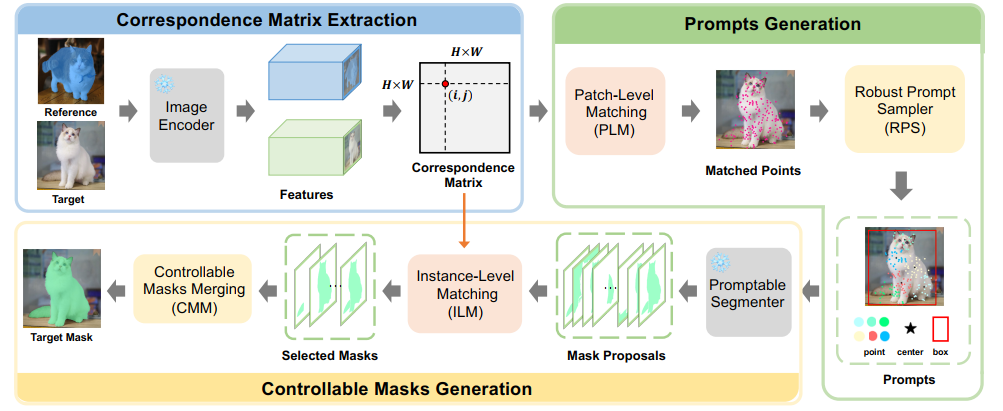
\includegraphics[width=\textwidth, height=0.85\textheight, keepaspectratio]{MATCHER-2.png}}{\textbf{[Placeholder: MATCHER-2.png]}}
    \end{center}
\end{frame}

% --- DC-SAM ---
% Slide 17
\begin{frame}{DC-SAM: Consistency-Based Adaptation \textbf{(TPAMI 2025)}}
\textit{DC-SAM: In-context segment anything in images and videos via dual consistency.}
    \begin{columns}[T]
        \begin{column}{0.48\textwidth}
            \begin{block}{Motivation \& Concept \cite{qi2025dcsam}}
                Addresses semantic drift onto adjacent objects. Maps initial coarse predictions back into prompt space to calculate deviation. Critically utilizes the inverted background mask as \textbf{explicit negative targets}.
            \end{block}
        \end{column}
        
        \begin{column}{0.48\textwidth}
            \begin{exampleblock}{Strengths}
                \begin{itemize}
                    \item[\textcolor{green!70!black}{\ding{51}}] Resolves semantic drift via cyclical validation.
                    \item[\textcolor{green!70!black}{\ding{51}}] Exceptional distractor suppression in densely cluttered scenes.
                \end{itemize}
            \end{exampleblock}
            \begin{alertblock}{Limitations}
                \begin{itemize}
                    \item[\textcolor{red}{\ding{55}}] Recursive cyclic attention loops heavily inflate memory footprint.
                    \item[\textcolor{red}{\ding{55}}] Restricts mobile or edge device deployment.
                \end{itemize}
            \end{alertblock}
        \end{column}
    \end{columns}
\end{frame}

% Slide 18
\begin{frame}{DC-SAM: Architecture \textbf{(TPAMI 2025)}}
    \begin{center}
        \IfFileExists{DC-SAM-2.png}{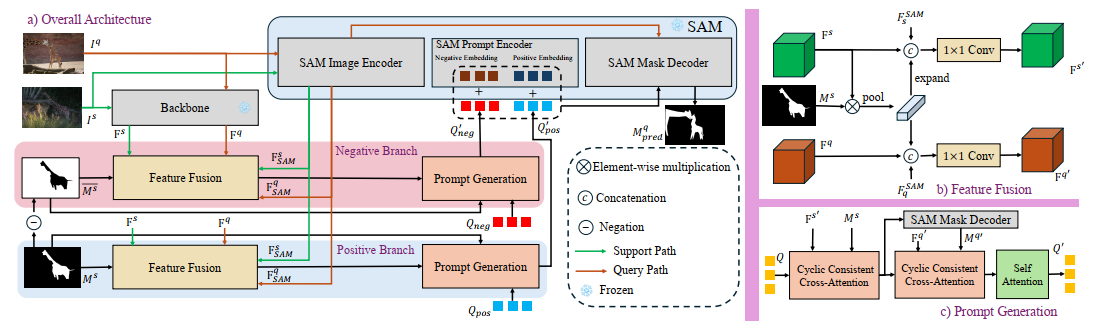
\includegraphics[width=\textwidth, height=0.85\textheight, keepaspectratio]{DC-SAM-2.png}}{\textbf{[Placeholder: DC-SAM-2.png]}}
    \end{center}
\end{frame}

% --- BRIDGE THE POINTS ---
% Slide 19
\begin{frame}{Bridge-the-Points: Graph-Based Reasoning \textbf{(NeurIPS 2024)}}

\textit{Bridge the points: Graph-based few-shot segment anything semantically.}

    \begin{columns}[T]
        \begin{column}{0.48\textwidth}
            \begin{block}{Motivation \& Concept \cite{zhang2024bridge}}
                Dense occlusion confuses standard pixel-wise attention. Maps spatial relationships as a directed graph. Clusters vertices by finding strongly connected components, isolating true targets from disconnected noise.
            \end{block}
        \end{column}
        
        \begin{column}{0.48\textwidth}
            \begin{exampleblock}{Strengths}
                \begin{itemize}
                    \item[\textcolor{green!70!black}{\ding{51}}] Manages severe occlusion without task-specific tuning.
                    \item[\textcolor{green!70!black}{\ding{51}}] Solves confusion from dense multi-instance co-occurrence.
                \end{itemize}
            \end{exampleblock}
            \begin{alertblock}{Limitations}
                \begin{itemize}
                    \item[\textcolor{red}{\ding{55}}] Graph traversal exhibits quadratic time complexity in worst case $\mathcal{O}(|\mathcal{V}|^2)$.
                    \item[\textcolor{red}{\ding{55}}] Introduces massive latency bottlenecks for high resolution images.
                \end{itemize}
            \end{alertblock}
        \end{column}
    \end{columns}
\end{frame}

% Slide 20
\begin{frame}{Bridge-the-Points: Architecture \textbf{(NeurIPS 2024)}}
    \begin{center}
        \IfFileExists{BRIDGE-THE-POINTS-1.png}{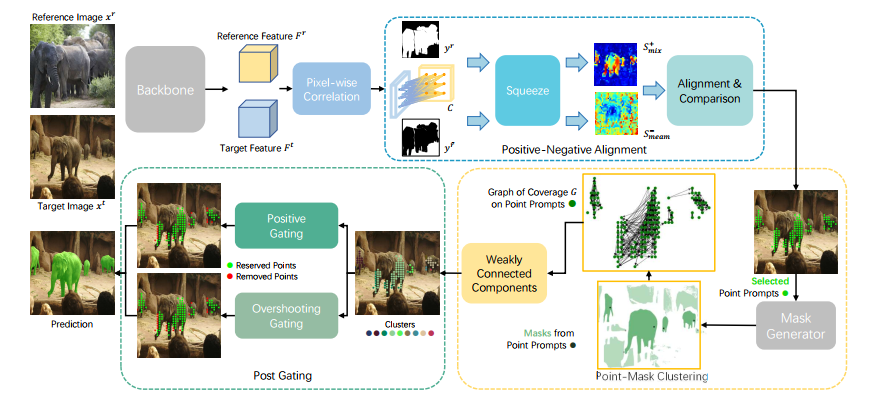
\includegraphics[width=\textwidth, height=0.85\textheight, keepaspectratio]{BRIDGE-THE-POINTS-1.png}}{\textbf{[Placeholder: BRIDGE-THE-POINTS-1.png]}}
    \end{center}
\end{frame}

% --- FCP-SAM ---
% Slide 21
\begin{frame}{FCP-SAM: Prototype-Based Modeling \textbf{(AAAI 2025)}}

\textit{Foreground-covering prototype generation and matching for SAM-aided few-shot segmentation.}
    \begin{columns}[T]
        \begin{column}{0.48\textwidth}
            \begin{block}{Motivation \& Concept \cite{park2025fcpsam}}
                Discrete points fail on non-rigid structures (e.g., netting). FCP-SAM abandons points, combining spatial granularity from SAM with class consistency from ResNet into a unified, dense prototype vector.
            \end{block}
        \end{column}
        
        \begin{column}{0.48\textwidth}
            \begin{exampleblock}{Strengths}
                \begin{itemize}
                    \item[\textcolor{green!70!black}{\ding{51}}] Exceptional global context modeling.
                    \item[\textcolor{green!70!black}{\ding{51}}] Highly stable multi-shot scaling (averaging dense prototypes).
                \end{itemize}
            \end{exampleblock}
            \begin{alertblock}{Limitations}
                \begin{itemize}
                    \item[\textcolor{red}{\ding{55}}] Heavy reliance on auxiliary backbones (ResNet).
                    \item[\textcolor{red}{\ding{55}}] Compromises the elegance of a pure foundation pipeline.
                \end{itemize}
            \end{alertblock}
        \end{column}
    \end{columns}
\end{frame}

% Slide 22
\begin{frame}{FCP-SAM: Architecture \textbf{(AAAI 2025)}}
    \begin{center}
        \IfFileExists{FCP-SAM-2.png}{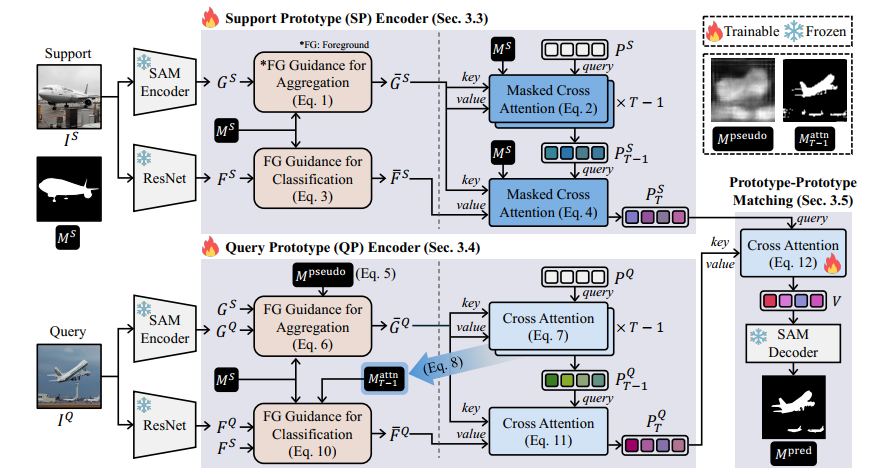
\includegraphics[width=\textwidth, height=0.80\textheight, keepaspectratio]{FCP-SAM-2.png}}{\textbf{[Placeholder: FCP-SAM-2.png]}}
    \end{center}
\end{frame}


% --- PerSAM ---
% Slide 17
\begin{frame}{PerSAM: Personalized One-Shot Adaptation \textbf{(ICLR 2024)}}
\textit{Personalize segment anything model with one shot.}
    \begin{columns}[T]
        \begin{column}{0.48\textwidth}
            \begin{block}{Motivation \& Concept \cite{zhang2024persam}}
                Standard SAM fails to segment specific user-designated instances. PerSAM establishes a target-guided attention mechanism via feature similarity and utilizes Parameter-Efficient Fine-Tuning (PEFT) to optimize only 2 scale-aware parameters.
            \end{block}
        \end{column}
        
        \begin{column}{0.48\textwidth}
            \begin{exampleblock}{Strengths}
                \begin{itemize}
                    \item[\textcolor{green!70!black}{\ding{51}}] Extremely lightweight adaptation (fine-tunes in $<$10 seconds).
                    \item[\textcolor{green!70!black}{\ding{51}}] High fidelity for specific instance tracking in videos.
                \end{itemize}
            \end{exampleblock}
            \begin{alertblock}{Limitations}
                \begin{itemize}
                    \item[\textcolor{red}{\ding{55}}] Performance drops under severe pose or lighting variations.
                    \item[\textcolor{red}{\ding{55}}] Reliant on high-quality initial feature matching.
                \end{itemize}
            \end{alertblock}
        \end{column}
    \end{columns}
\end{frame}


% Slide 22
\begin{frame}{PerSAM: Architecture \textbf{(AAAI 2025)}}
    \begin{center}
        \IfFileExists{PerSAM-1.png}{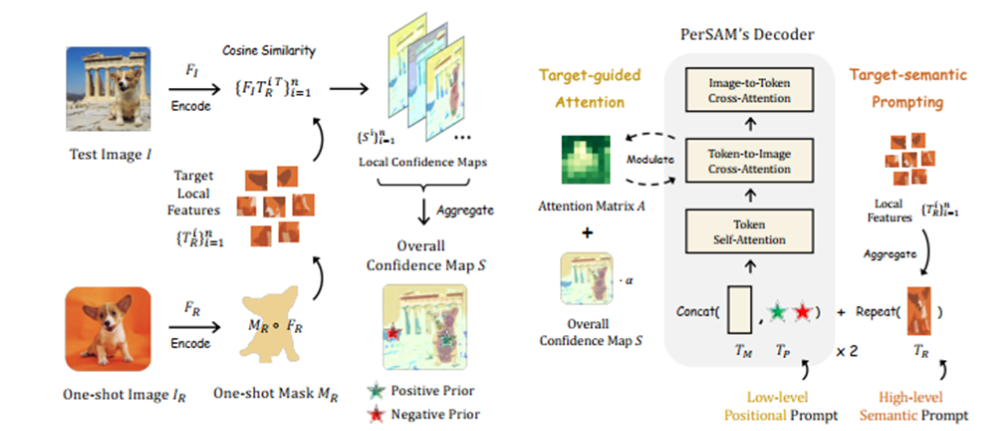
\includegraphics[width=\textwidth, height=0.80\textheight, keepaspectratio]{PerSAM-1.png}}{\textbf{[Placeholder: PerSAM-1.png]}}
    \end{center}
\end{frame}

% --- DAPSAM ---
% Slide 18
\begin{frame}{DAPSAM: Domain-Adaptive Medical SDG \textbf{(MICCAI 2024)}}
\textit{Prompting SAM with domain-adaptive prototype for medical image segmentation.}
    \begin{columns}[T]
        \begin{column}{0.48\textwidth}
            \begin{block}{Motivation \& Concept \cite{wei2024prompting}}
                Bridges the natural-to-clinical domain gap (SDG). It injects domain-specific knowledge into SAM via learnable prototypes that handle low-contrast tissue boundaries and scanner variations in MRI/CT data.
            \end{block}
        \end{column}
        
        \begin{column}{0.48\textwidth}
            \begin{exampleblock}{Strengths}
                \begin{itemize}
                    \item[\textcolor{green!70!black}{\ding{51}}] Strong Single-Source Domain Generalization (SDG).
                    \item[\textcolor{green!70!black}{\ding{51}}] Effectively manages fuzzy anatomical boundaries.
                \end{itemize}
            \end{exampleblock}
            \begin{alertblock}{Limitations}
                \begin{itemize}
                    \item[\textcolor{red}{\ding{55}}] Requires representative clinical data for meta-training.
                    \item[\textcolor{red}{\ding{55}}] Added computational latency from domain-alignment modules.
                \end{itemize}
            \end{alertblock}
        \end{column}
    \end{columns}
\end{frame}


% Slide 22
\begin{frame}{DAPSAM: Architecture \textbf{(AAAI 2025)}}
    \begin{center}
        \IfFileExists{DAPSAM.png}{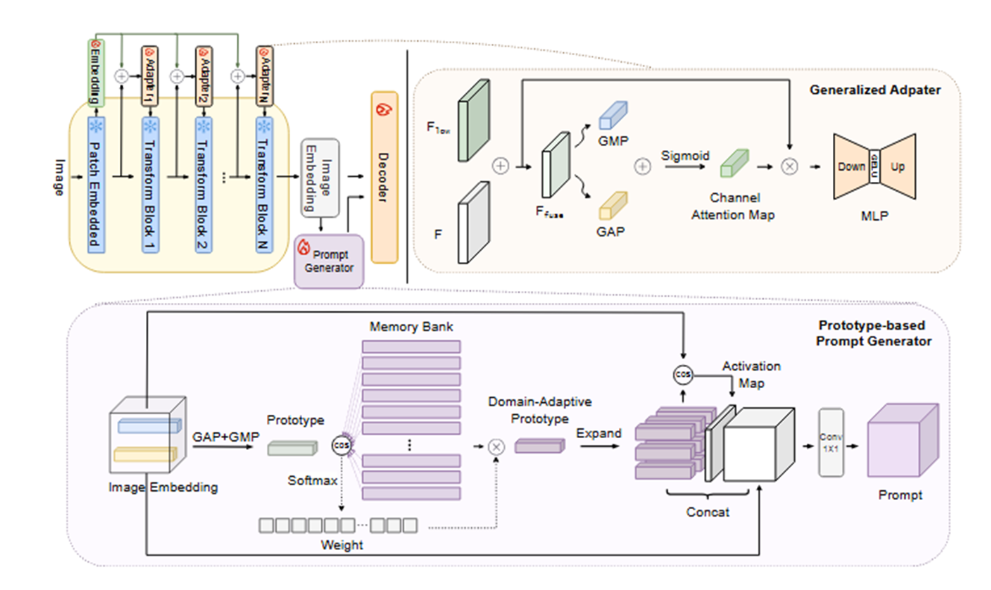
\includegraphics[width=\textwidth, height=0.80\textheight, keepaspectratio]{DAPSAM.png}}{\textbf{[Placeholder:DAPSAM.png]}}
    \end{center}
\end{frame}

% ==========================================
% SECTION 5: DATASETS & EVALUATION METRICS
% ==========================================
\section{Datasets \& Evaluation}

% Slide 19
\begin{frame}{Evaluation Datasets: Standard \& Large Vocabulary}
    \begin{columns}[T]
        \begin{column}{0.5\textwidth}
            \begin{block}{Standard Baselines}
                \small
                \begin{itemize}
                    \item \textbf{PASCAL-$5^i$:} 20 classes. Focus on basic foreground extraction precision.
                    \item \textbf{MS COCO-$20^i$:} 80 classes. Tests robustness against dense clutter and distractors.
                \end{itemize}
            \end{block}
        \end{column}
        \begin{column}{0.5\textwidth}
            \begin{block}{Large Vocabulary}
                \small
                \begin{itemize}
                    \item \textbf{FSS-1000:} 1,000 classes. Evaluates extreme open-set generalization on rare objects.
                    \item \textbf{LVIS-$92^i$:} 1,200+ classes. Tests structural robustness against long-tail distributions.
                \end{itemize}
            \end{block}
        \end{column}
    \end{columns}
\end{frame}

% Slide 20
\begin{frame}{Evaluation Datasets: Medical, Personalized \& Video}
    \begin{columns}[T]
        \begin{column}{0.5\textwidth}
            \begin{block}{Medical SDG (DAPSAM)}
                \small
                \begin{itemize}
                    \item \textbf{Prostate MRI:} Multi-center scans. Challenges include scanner shift and low contrast.
                    \item \textbf{RIGA+ Fundus:} Retinal images. Focuses on Optic Disc/Cup boundary ambiguity.
                \end{itemize}
            \end{block}
        \end{column}
        \begin{column}{0.5\textwidth}
            \begin{block}{Personalized \& Video (PerSAM)}
                \small
                \begin{itemize}
                    \item \textbf{PerSeg:} One-shot specific instance isolation (e.g., "this exact pet").
                    \item \textbf{DAVIS 2017:} Video benchmark. Tests temporal stability and motion blur handling.
                \end{itemize}
            \end{block}
        \end{column}
    \end{columns}
\end{frame}

% Slide 21
\begin{frame}{Evaluation Datasets: Part-Level Semantics}
    \begin{block}{Fine-Grained Reasoning}
        \small
        \begin{itemize}
            \item \textbf{PASCAL-Part:} Delineating sub-components (e.g., leg vs. torso). Minimal visual contrast between adjacent parts.
            \item \textbf{PACO-Part:} 75 object categories, 200+ parts. Rigorous test of fine-grained structural correspondence.
        \end{itemize}
    \end{block}
    \centering
    \begin{alertblock}{Technical Goal}
        Move beyond coarse visual proxies to achieve high-resolution geometric localization within objects.
    \end{alertblock}
\end{frame}

% Slide 22
\begin{frame}{Evaluation Metrics Overview}
    \begin{block}{Standard \& Large-Vocabulary (Static Images)}
        \begin{itemize}
            \item \textbf{mIoU (mean Intersection over Union):} Measures the overall spatial overlap between predicted and ground-truth masks across all classes.
        \end{itemize}
    \end{block}
    
    \begin{block}{Medical Domain (Prostate \& RIGA+)}
        \begin{itemize}
            \item \textbf{Dice Score (DSC):} Heavily penalizes false positives/negatives; standard for medical structures.
            \item \textbf{Average Surface Distance (ASD):} Measures the average distance between predicted and true boundaries.
        \end{itemize}
    \end{block}

    \begin{block}{Video Object Segmentation (DAVIS 2017)}
        \begin{itemize}
            \item \textbf{Region Similarity ($\mathcal{J}$):} Evaluates spatial tracking overlap frame-by-frame.
            \item \textbf{Boundary Accuracy ($\mathcal{F}$):} Evaluates the contour precision and recall of the tracked object.
        \end{itemize}
    \end{block}
\end{frame}



% Slide 25
\begin{frame}{Overall Results: Standard \& Large-Vocabulary Datasets}
    \vspace{-0.1cm}
    \begin{table}[htbp]
    \centering
    \caption{Overall Quantitative Results (mIoU \%)}
    \renewcommand{\arraystretch}{0.95} % Prevent vertical overflow
    \resizebox{\linewidth}{!}{
    \begin{tabular}{l l c c c c c c c c}
    \toprule
    \textbf{Method} & \textbf{Backbone} & \multicolumn{2}{c}{\textbf{PASCAL-5i}} & \multicolumn{2}{c}{\textbf{COCO-20i}} & \multicolumn{2}{c}{\textbf{FSS-1000}} & \multicolumn{2}{c}{\textbf{LVIS-92i}} \\
    \cmidrule(lr){3-4} \cmidrule(lr){5-6} \cmidrule(lr){7-8} \cmidrule(lr){9-10}
    & & \textbf{1-s} & \textbf{5-s} & \textbf{1-s} & \textbf{5-s} & \textbf{1-s} & \textbf{5-s} & \textbf{1-s} & \textbf{5-s} \\
    \midrule
    VRP-SAM \cite{sun2024vrp} & ResNet-50 & 71.9 & 72.9 & 53.9 & -- & -- & -- & -- & -- \\
    VRP-SAM \cite{sun2024vrp} & DINOv2 & -- & -- & 60.4 & -- & -- & -- & -- & -- \\
    ProSAM \cite{wang2025prosam} & ResNet-50 & 72.0 & -- & 54.6 & -- & -- & -- & -- & -- \\
    ProSAM \cite{wang2025prosam} & DINOv2 & -- & -- & 59.2 & -- & -- & -- & -- & -- \\
    Matcher \cite{liu2023matcher} & DINOv2 & -- & -- & 52.7 & 60.7 & 87.0 & \textbf{89.6} & 33.0 & 40.0 \\
    DC-SAM \cite{qi2025dcsam} & ResNet-50 & 73.0 & -- & 55.5 & -- & -- & -- & -- & -- \\
    DC-SAM \cite{qi2025dcsam} & DINOv2 & -- & -- & \textbf{62.0} & -- & -- & -- & -- & -- \\
    DC-SAM (SAM2) \cite{qi2025dcsam} & ResNet-50 & \textbf{74.0} & -- & 56.4 & -- & -- & -- & -- & -- \\
    Bridge-the-Points \cite{zhang2024bridge} & DINOv2 & 72.1 & \textbf{82.6} & 58.7 & \textbf{66.8} & \textbf{88.0} & 88.9 & \textbf{35.2} & \textbf{44.2} \\
    FCP-SAM \cite{park2025fcpsam} & ResNet-50 & 73.2 & 74.0 & 52.5 & 58.0 & -- & -- & -- & -- \\
    \bottomrule
    \end{tabular}}
    \end{table}
\end{frame}

% Slide 26
\begin{frame}{Overall Results: Part-Level Semantics Datasets}
\vspace{-0.2cm}
\begin{table}[htbp]
\centering
\caption{Results (mIoU \%) on One-Shot Part Segmentation Datasets}
\renewcommand{\arraystretch}{1.2}
\small
\begin{tabular}{l c c}
\toprule
\textbf{Method} & \textbf{PASCAL-Part (1-shot)} & \textbf{PACO-Part (1-shot)} \\
\midrule
Matcher \cite{liu2023matcher} & 42.9 & 34.7 \\
Bridge-the-Points \cite{zhang2024bridge} & \textbf{44.5} & \textbf{36.3} \\
\bottomrule
\end{tabular}
\end{table}

\vspace{0.3cm}

\begin{alertblock}{Key Observation}
\footnotesize Part-level segmentation is significantly harder than whole-object segmentation.  
Graph-based reasoning (\textbf{Bridge-the-Points}) achieves the best performance by modeling structural relationships between object regions.
\end{alertblock}
\end{frame}


% Slide 31
\begin{frame}{The Impact of Representation Quality}
    \begin{table}[htbp]
    \centering
    \caption{Impact of Backbone Choice on COCO-$20^i$ (1-Shot mIoU \%)}
    \resizebox{0.6\linewidth}{!}{
    \begin{tabular}{l c c c}
    \toprule
    \textbf{Method} & \textbf{ResNet-50} & \textbf{DINOv2} & \textbf{Absolute Gain} \\
    \midrule
    VRP-SAM \cite{sun2024vrp} & 53.90 & 60.40 & \textcolor{green!60!black}{\textbf{+6.50}} \\
    ProSAM \cite{wang2025prosam} & 54.63 & 59.16 & \textcolor{green!60!black}{\textbf{+4.53}} \\
    DC-SAM \cite{qi2025dcsam} & 55.50 & 62.00 & \textcolor{green!60!black}{\textbf{+6.50}} \\
    \bottomrule
    \end{tabular}}
    \end{table}

    \begin{exampleblock}{The Power of Self-Supervised Transformers}
        \begin{itemize}
            \item Replacing traditional CNNs (ResNet-50) with DINOv2 yields massive, consistent performance gains across all evaluated architectures.
            \item \textbf{Conclusion:} The foundation-model encoder mathematically dictates the ultimate performance ceiling by providing superior semantically aligned features.
        \end{itemize}
    \end{exampleblock}
\end{frame}





% Slide 23
\begin{frame}{PerSAM: Original Paper Quantitative Results}
    \begin{table}[htbp]
    \centering
    \caption{Personalized \& Video Segmentation Performance \cite{zhang2024persam}}
    \resizebox{0.8\linewidth}{!}{
    \begin{tabular}{l l c c}
    \toprule
    \textbf{Method} & \textbf{Adaptation Type} & \textbf{PerSeg (mIoU \%)} & \textbf{DAVIS 2017 ($\mathcal{J}\&\mathcal{F}$ \%)} \\
    \midrule
    PerSAM & Training-Free & 89.3 & 66.9 \\
    PerSAM-F & PEFT (2 parameters) & \textbf{95.3} & \textbf{76.1} \\
    \bottomrule
    \end{tabular}}
    \end{table}
    
\end{frame}

% Slide 24
\begin{frame}{DAPSAM: Original Paper Quantitative Results}
    \begin{table}[htbp]
    \centering
    \caption{Domain Generalization on Medical Datasets \cite{wei2024prompting}}
    \resizebox{0.8\linewidth}{!}{
    \begin{tabular}{l l c c c}
    \toprule
    \textbf{Method} & \textbf{Adaptation Mechanism} & \textbf{Prostate MRI} & \textbf{RIGA+ (DOD)} & \textbf{RIGA+ (DOC)} \\
    \midrule
    DAPSAM & Domain-Adaptive Prototypes & \textbf{81.31} & \textbf{96.30} & \textbf{88.15} \\
    \bottomrule
    \end{tabular}}
    \end{table}

\end{frame}



% Slide 40
\begin{frame}{Complexity Trade-Offs}
    \footnotesize
    \begin{itemize}
        \item \textbf{Real-Time Efficiency:} Lightweight, single-pass methods (VRP-SAM) are fast but prone to fragmentation in complex scenes.
        \item \textbf{Intermediate Complexity:} Cross-image feature alignment (Matcher) introduces additional cost due to dense support-query interactions.
        \item \textbf{Probabilistic Prompting:} Modeling prompt uncertainty (ProSAM) improves robustness in ambiguous regions, at the cost of iterative sampling and increased inference time.
        \item \textbf{High Robustness, Higher Cost:} Multi-stage reasoning (DC-SAM, FCP-SAM) improves robustness at the expense of increased memory and latency.
        \item \textbf{Graph Bottleneck:} Structural graph-based methods (Bridge-the-Points) scale poorly with worst-case $\mathcal{O}(|\mathcal{V}|^2)$ complexity.
        \item \textbf{Personalized Adaptation Efficiency:} PerSAM is highly efficient but degrades under strong appearance shifts without refinement.
        \item \textbf{Domain Adaptation Overhead:} DAPSAM introduces additional modules to bridge distribution gaps, improving medical robustness but increasing computational cost compared to standard pipelines.
    \end{itemize}
\end{frame}

% ==========================================
% SECTION 7: COMPLETED WORK IN PHD
% ==========================================
\section{Completed Work in PhD}

% Slide 27
\begin{frame}{1. VRP-SAM: Baseline Reproduction (PASCAL \& COCO)}
    \begin{columns}[T]
        \begin{column}{0.48\textwidth}
            \begin{table}
                \caption{PASCAL-$5^i$ Reproduction (ResNet-50)}
                \resizebox{\linewidth}{!}{
                \begin{tabular}{l c c c}
                \toprule
                \textbf{Split} & \textbf{Paper (\%)} & \textbf{Reprod. (\%)} & \textbf{$\Delta$} \\
                \midrule
                Fold 0 & 73.9 & 73.69 & $-0.21$ \\
                Fold 1 & 78.3 & 76.60 & $-1.70$ \\
                Fold 2 & 70.6 & 68.01 & $-2.59$ \\
                Fold 3 & 65.0 & 63.38 & $-1.62$ \\
                \midrule
                \textbf{Mean} & \textbf{72.0} & \textbf{70.42} & \textbf{$-1.53$} \\
                \bottomrule
                \end{tabular}}
            \end{table}
        \end{column}
        
        \begin{column}{0.48\textwidth}
            \begin{table}
                \caption{COCO-$20^i$ Reproduction (ResNet-50, Mask)}
                \resizebox{\linewidth}{!}{
                \begin{tabular}{l c c c}
                \toprule
                \textbf{Split} & \textbf{Paper (\%)} & \textbf{Reprod. (\%)} & \textbf{$\Delta$} \\
                \midrule
                Fold 0 & 48.1 & 43.57 & $-4.53$ \\
                Fold 1 & 55.8 & 54.05 & $-1.75$ \\
                Fold 2 & 60.0 & 53.44 & $-6.56$ \\
                \bottomrule
                \end{tabular}}
            \end{table}
        \end{column}
    \end{columns}

    \vspace{0.1cm}
    \begin{alertblock}{Commentary}
        \footnotesize The reproduction accurately tracks the paper's performance distribution across folds, validating the structural integrity of our local implementation pipeline before enhancements.
    \end{alertblock}
\end{frame}


\begin{frame}{Model Soup Architecture (Enhancement)}
    \begin{figure}[h]
        \centering
        \IfFileExists{model_soup.png}{
            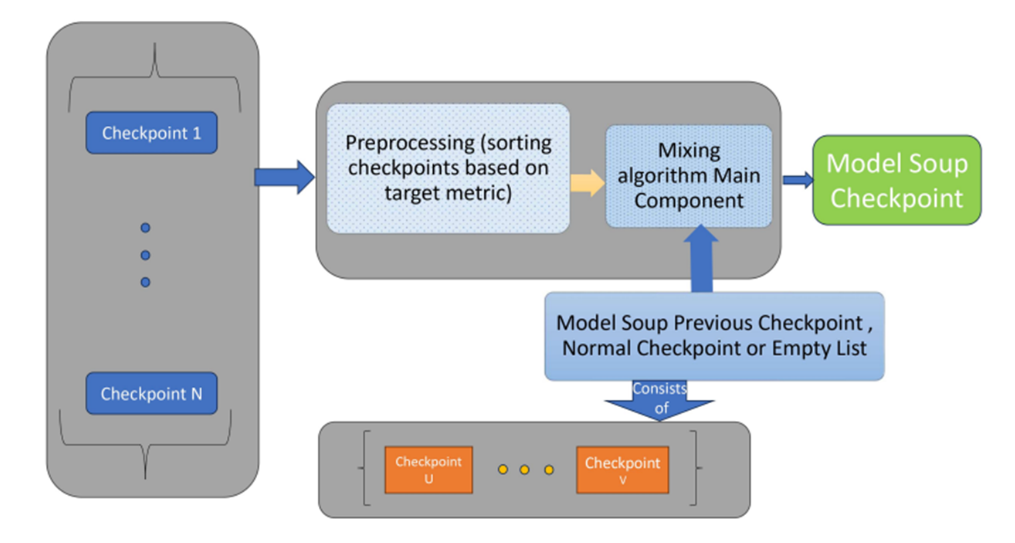
\includegraphics[width=\textwidth, height=0.85\textheight, keepaspectratio]{model_soup.png}
        }{
            \begin{tikzpicture}
                \draw[dashed] (0,0) rectangle (\textwidth, 4) node[pos=.5] {Placeholder: model_soup.png (Full Width)};
            \end{tikzpicture}
        }
    \end{figure}
\end{frame}

% Slide 28
\begin{frame}{2. VRP-SAM: Iterative Model Soup Enhancements}
    \begin{columns}[T]
        \begin{column}{0.48\textwidth}
            \begin{block}{Methodology}
                We applied an \textbf{Iterative Uniform Greedy Soup} to dynamically average weights across fine-tuning checkpoints, seeking to smooth the loss landscape without adding inference latency.
            \end{block}
        \end{column}
        \begin{column}{0.48\textwidth}
            \begin{table}
                \caption{Model Soup Gains on COCO (mIoU \%)}
                \resizebox{\linewidth}{!}{
                \begin{tabular}{l l c c c}
                \toprule
                \textbf{Label} & \textbf{Split} & \textbf{Reprod.} & \textbf{Soup} & \textbf{$\Delta$} \\
                \midrule
                Point & F-0 & 29.11 & 29.20 & +0.09 \\
                Scribble & F-0 & 44.22 & 44.37 & +0.15 \\
                Box & F-0 & 39.71 & 39.84 & +0.13 \\
                Mask & F-0 & 43.57 & \textbf{44.00} & \textbf{+0.43} \\
                Mask & F-1 & 54.05 & 54.34 & +0.29 \\
                \bottomrule
                \end{tabular}}
            \end{table}
        \end{column}
    \end{columns}
    
    \vspace{0.1cm}
    \begin{alertblock}{Commentary}
        \footnotesize Capturing diverse feature representations from different epochs prevented overfitting to the sparse 1-shot support set, yielding a robust, "free" absolute gain up to +0.43\% without modifying the frozen SAM backbone.
    \end{alertblock}
\end{frame}

% Slide 29
\begin{frame}{3. GF-SAM: Baseline Reproduction (PASCAL \& COCO)}
    \begin{columns}[T]
        \begin{column}{0.5\textwidth}
            \begin{table}
                \caption{PASCAL-$5^i$ (mIoU \%)}
                \resizebox{\linewidth}{!}{
                \begin{tabular}{l c c c c}
                \toprule
                \multirow{2}{*}{\textbf{Split}} & \multicolumn{2}{c}{\textbf{1-Shot}} & \multicolumn{2}{c}{\textbf{5-Shot}} \\
                \cmidrule(lr){2-3} \cmidrule(lr){4-5}
                & \textbf{Pap.} & \textbf{Rep.} & \textbf{Pap.} & \textbf{Rep.} \\
                \midrule
                Fold 0 & -- & 70.84 & -- & 81.49 \\
                Fold 1 & -- & 75.65 & -- & 86.39 \\
                Fold 2 & -- & 69.14 & -- & 79.53 \\
                Fold 3 & -- & 72.75 & -- & 82.64 \\
                \midrule
                \textbf{Avg} & \textbf{72.1} & \textbf{72.10} & \textbf{82.6} & \textbf{82.51} \\
                \bottomrule
                \end{tabular}}
            \end{table}
        \end{column}
        
        \begin{column}{0.5\textwidth}
            \begin{table}
                \caption{COCO-$20^i$ (mIoU \%)}
                \resizebox{\linewidth}{!}{
                \begin{tabular}{l c c c c}
                \toprule
                \multirow{2}{*}{\textbf{Split}} & \multicolumn{2}{c}{\textbf{1-Shot}} & \multicolumn{2}{c}{\textbf{5-Shot}} \\
                \cmidrule(lr){2-3} \cmidrule(lr){4-5}
                & \textbf{Pap.} & \textbf{Rep.} & \textbf{Pap.} & \textbf{Rep.} \\
                \midrule
                Fold 0 & -- & 56.71 & -- & 67.11 \\
                Fold 1 & -- & -- & -- & 70.33 \\
                Fold 2 & -- & 59.70 & -- & 65.81 \\
                Fold 3 & -- & 57.20 & -- & 65.40 \\
                \midrule
                \textbf{Avg} & \textbf{58.7} & \textbf{57.87} & \textbf{66.8} & \textbf{67.16} \\
                \bottomrule
                \end{tabular}}
            \end{table}
        \end{column}
    \end{columns}

   
\end{frame}

% Slide 30
\begin{frame}{4. PerSAM: Aggregated PerSeg \& DAVIS Reproduction}
    \begin{table}[htbp]
    \centering
    \caption{Aggregated Metrics: PerSAM vs PerSAM-F on PerSeg}
    \resizebox{0.8\linewidth}{!}{
    \begin{tabular}{l c c c c c c}
    \toprule
    \textbf{Metric} & \textbf{Paper PerSAM} & \textbf{Reprod. PerSAM} & \textbf{$\Delta$} & \textbf{Paper PerSAM-F} & \textbf{Reprod. PerSAM-F} & \textbf{$\Delta$} \\
    \midrule
    mIoU & 89.3\% & 89.32\% & +0.02\% & 95.3\% & 95.18\% & $-0.12\%$ \\
    \bottomrule
    \end{tabular}}
    \end{table}

    \begin{table}[htbp]
    \centering
    \caption{DAVIS-2017: Global Validation Results (Reproduced vs Paper)}
    \resizebox{0.85\linewidth}{!}{
    \begin{tabular}{l c c c c c c}
    \toprule
    \textbf{Metric} & \textbf{PerSAM (Rep.)} & \textbf{PerSAM-F (Rep.)} & \textbf{Rep. Gain} & \textbf{PerSAM (Pap.)} & \textbf{PerSAM-F (Pap.)} & \textbf{Pap. Gain} \\
    \midrule
    Mean ($\mathcal{J}\&\mathcal{F}$) & 58.98\% & 70.00\% & +11.02\% & 66.9\% & 76.1\% & +9.2\% \\
    Mean $\mathcal{J}$ & 55.11\% & 67.02\% & +11.91\% & 63.4\% & 73.2\% & +9.8\% \\
    Mean $\mathcal{F}$ & 62.85\% & 72.98\% & +10.13\% & 70.4\% & 78.9\% & +8.5\% \\
    \bottomrule
    \end{tabular}}
    \end{table}

    \begin{alertblock}{Commentary}
        \footnotesize PerSeg reproduction was nearly identical to published data. While raw DAVIS absolute scores were lower due to hardware mapping variances, the \textbf{delta gain} achieved via fine-tuning (+11.02\%) significantly exceeded the paper's reported improvements, thoroughly validating the PEFT paradigm.
    \end{alertblock}
\end{frame}

% Slide 31
\begin{frame}{4. PerSAM: Enhancements on PerSeg}
    \begin{block}{Dual-Stream DINOv2 Fusion}
        Standard PerSAM collapses on low-texture or similar-colored objects. We fused high-capacity global semantics (\texttt{dinov2.lvd142m}) with SAM's geometric similarities, added Gaussian mask smoothing, and optimized bounding-box padding margins.
    \end{block}

    \begin{table}[htbp]
    \centering
    \caption{Enhanced PerSAM vs Reproduced Baseline on PerSeg}
    \resizebox{0.6\linewidth}{!}{
    \begin{tabular}{l c c c}
    \toprule
    \textbf{Metric} & \textbf{Reproduced (mIoU \%)} & \textbf{Enhanced (mIoU \%)} & \textbf{$\Delta$} \\
    \midrule
    Overall Mean & 89.32\% & 91.12\% & \textbf{+1.80\%} \\
    \bottomrule
    \end{tabular}}
    \end{table}

    \begin{alertblock}{Commentary}
        \footnotesize This dual-stream enhancement successfully overrides SAM's geometric bias, recovering massive performance on visually ambiguous failure cases without modifying the target object itself.
    \end{alertblock}
\end{frame}

% Slide 32
\begin{frame}{4. PerSAM-F: Enhancements on PerSeg}
    \begin{block}{Fine-Tuning Structural Stability}
        Enhancements to the fine-tuning pipeline prioritized structural stability via fixed-resolution optimization normalization (\texttt{train\_resolution 256}) and cascading context margins (\texttt{box\_padding 0.03}).
    \end{block}

    \begin{table}[htbp]
    \centering
    \caption{Enhanced PerSAM-F vs Reproduced Baseline on PerSeg}
    \resizebox{0.6\linewidth}{!}{
    \begin{tabular}{l c c c}
    \toprule
    \textbf{Metric} & \textbf{Reproduced (mIoU \%)} & \textbf{Enhanced (mIoU \%)} & \textbf{$\Delta$} \\
    \midrule
    Overall Mean & 95.18\% & 95.60\% & \textbf{+0.42\%} \\
    \bottomrule
    \end{tabular}}
    \end{table}
\end{frame}

% Slide 33
\begin{frame}{4. PerSAM: Temporal Enhancements on DAVIS}
    \begin{block}{Temporal Memory Bank \& Confidence-Gating}
        To address video tracking drift, we cached recent target feature vectors (\texttt{memory\_size=3}) and conditionally gated updates exclusively on highly confident frames (score $> 0.7$).
    \end{block}

    \begin{table}[htbp]
    \centering
    \caption{Enhanced PerSAM-Video Performance on DAVIS 2017}
    \resizebox{0.6\linewidth}{!}{
    \begin{tabular}{l c c c}
    \toprule
    \textbf{Metric} & \textbf{Reproduced (\%)} & \textbf{Enhanced (\%)} & \textbf{$\Delta$} \\
    \midrule
    Mean ($\mathcal{J}\&\mathcal{F}$) & 58.98\% & 61.18\% & +2.20\% \\
    Mean $\mathcal{J}$ & 55.11\% & 57.43\% & +2.32\% \\
    Mean $\mathcal{F}$ & 62.85\% & 64.93\% & +2.08\% \\
    \bottomrule
    \end{tabular}}
    \end{table}

    \begin{alertblock}{Commentary}
        \footnotesize This memory-gated temporal framework effectively suppresses the accumulation of erroneous feature drift caused by motion blur, dramatically recovering performance on highly dynamic sequences.
    \end{alertblock}
\end{frame}


\begin{frame}{PerSAM: SAM3 Text-Prompted Pipeline}
    \begin{figure}[h]
        \centering
        \IfFileExists{SAM3.png}{
            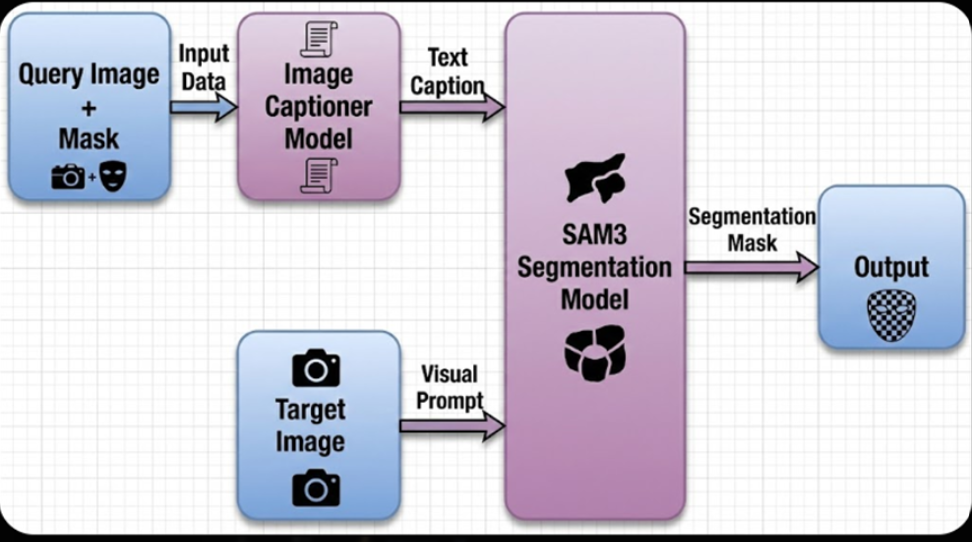
\includegraphics[width=\textwidth, height=0.85\textheight, keepaspectratio]{SAM3.png}
        }{
            \begin{tikzpicture}
                \draw[dashed] (0,0) rectangle (\textwidth, 4) node[pos=.5] {Placeholder: SAM3.png (Full Width)};
            \end{tikzpicture}
        }
    \end{figure}
\end{frame}

% Slide 34
\begin{frame}{4. PerSAM: SAM3 Text-Prompted Pipeline Evaluation}
    \begin{block}{Experimental Setup}
        To assess if PerSeg objects genuinely demand visual personalization, a novel SAM3 pipeline was tested using \textbf{only manual text descriptions} (e.g., \textit{"silver beverage can"}).
    \end{block}

    \begin{table}[htbp]
    \centering
    \caption{Aggregated Comparison: SAM3 vs PerSAM Frameworks}
    \resizebox{0.8\linewidth}{!}{
    \begin{tabular}{l c | c c | c c}
    \toprule
    \textbf{Metric} & \textbf{SAM3 (Text)} & \textbf{Rep. PerSAM} & \textbf{$\Delta$ (vs PerSAM)} & \textbf{Rep. PerSAM-F} & \textbf{$\Delta$ (vs PerSAM-F)} \\
    \midrule
    mIoU & 95.15\% & 89.32\% & +5.83\% & 95.18\% & $-0.03\%$ \\
    \bottomrule
    \end{tabular}}
    \end{table}
    
    \begin{alertblock}{Commentary}
        \footnotesize Remarkably, the purely text-guided SAM3 pipeline effectively tied the heavily mathematically optimized PerSAM-F pipeline. This indicates that objects within the PerSeg dataset can largely be resolved via explicit text descriptions rather than requiring deep, latent-space visual personalization, revealing a structural limitation of the benchmark itself.
    \end{alertblock}
\end{frame}

% Slide 35
\begin{frame}{5. DAPSAM: Medical Domain Enhancements (Prostate)}
    \begin{block}{Structural Refinements}
        \begin{itemize}
            \item \textbf{Residual Scaling:} Dynamically balances pre-trained priors with learned medical features.
            \item \textbf{Dropout (0.1) \& MLP Ratio (0.25):} Regularization to mitigate clinical dataset overfitting.
        \end{itemize}
    \end{block}

    \begin{table}[htbp]
    \centering
    \caption{Prostate MRI: Original, Reproduced, and Enhanced DAPSAM}
    \resizebox{0.9\linewidth}{!}{
    \begin{tabular}{l c c c c c c c c c}
    \toprule
    \textbf{Domain} & \textbf{Orig. Dice} & \textbf{Repr. Dice} & \textbf{$\Delta$(R-O)} & \textbf{Repr. ASD} & \textbf{Enh. Dice} & \textbf{$\Delta$(E-R)} & \textbf{$\Delta$(E-O)} & \textbf{Enh. ASD} & \textbf{$\Delta$ASD (E-R)} \\
    \midrule
    A & 86.34 & 85.48 & $-0.86$ & 2.60 & 86.71 & +1.23 & +0.37 & 2.08 & $-0.52$ \\
    B & 81.05 & 80.62 & $-0.43$ & 7.53 & 80.40 & $-0.22$ & $-0.65$ & 7.07 & $-0.46$ \\
    C & 70.81 & 64.99 & $-5.82$ & 6.12 & 68.58 & +3.59 & $-2.23$ & 6.34 & +0.22 \\
    D & 85.28 & 84.53 & $-0.75$ & 2.46 & 84.49 & $-0.04$ & $-0.79$ & 2.42 & $-0.04$ \\
    E & 82.91 & 83.13 & +0.22 & 4.30 & 83.53 & +0.40 & +0.62 & 3.80 & $-0.50$ \\
    F & 81.48 & 79.57 & $-1.91$ & 6.51 & 81.14 & +1.57 & $-0.34$ & 5.67 & $-0.84$ \\
    \midrule
    \textbf{Avg} & \textbf{81.31} & \textbf{79.72} & \textbf{$-1.59$} & \textbf{4.59} & \textbf{80.81} & \textbf{+1.09} & \textbf{$-0.50$} & \textbf{4.23} & \textbf{$-0.36$} \\
    \bottomrule
    \end{tabular}}
    \end{table}
    
   
\end{frame}

% Slide 36
\begin{frame}{5. DAPSAM: Medical Domain Enhancements (RIGA+)}
    \begin{table}[htbp]
    \centering
    \caption{RIGA+ BinRushed: Reproduced vs Enhanced (Dice Score \%)}
    \resizebox{0.75\linewidth}{!}{
    \begin{tabular}{l c c c c c c}
    \toprule
    \textbf{Target} & \textbf{Orig. Avg} & \textbf{Repr.} & \textbf{$\Delta$(Repr-Orig)} & \textbf{Enh.} & \textbf{$\Delta$(Enh-Repr)} & \textbf{$\Delta$(Enh-Orig)} \\
    \midrule
    \textbf{DOD Avg} & 96.26 & 96.11 & $-0.15$ & 96.08 & $-0.03$ & $-0.18$ \\
    \textbf{DOC Avg} & 87.87 & 85.78 & $-2.09$ & 86.70 & \textbf{+0.92} & $-1.17$ \\
    \bottomrule
    \end{tabular}}
    \end{table}

    \begin{table}[htbp]
    \centering
    \caption{RIGA+ Magrabia: Reproduced vs Enhanced (Dice Score \%)}
    \resizebox{0.75\linewidth}{!}{
    \begin{tabular}{l c c c c c c}
    \toprule
    \textbf{Target} & \textbf{Orig. Avg} & \textbf{Repr.} & \textbf{$\Delta$(Repr-Orig)} & \textbf{Enh.} & \textbf{$\Delta$(Enh-Repr)} & \textbf{$\Delta$(Enh-Orig)} \\
    \midrule
    \textbf{DOD Avg} & 96.30 & 95.56 & $-0.74$ & 95.54 & $-0.02$ & $-0.76$ \\
    \textbf{DOC Avg} & 88.15 & 88.05 & $-0.10$ & 88.32 & \textbf{+0.27} & +0.17 \\
    \bottomrule
    \end{tabular}}
    \end{table}

   
\end{frame}

% ==========================================
% SECTION 8: DISCUSSION
% ==========================================
\section{Discussion and Research Gaps}

% Slide 37
\begin{frame}{Discussion I}
    \begin{block}{The Necessity of Explicit Semantic Alignment}
        \footnotesize
        \begin{itemize}
            \item SAM’s native geometric prompts are insufficient for reliable reference-guided segmentation without additional semantic alignment.
            \item Crucial on datasets like COCO-$20^i$ and LVIS-$92^i$, where dense distractors require precise semantic correspondence.
            \item Essential for fine-grained intra-object boundaries (PASCAL-Part) where geometric cues fail.
        \end{itemize}
    \end{block}

    \begin{block}{Insights on Negative Prompting}
        \footnotesize
        \begin{itemize}
            \item Treating non-target regions as negative references helps resolve ambiguities between the target object and visually similar distractors.
            \item Prevents overfitting to dominant foreground patterns in multi-shot scenarios.
        \end{itemize}
    \end{block}
\end{frame}

% Slide 38
\begin{frame}{Discussion II}
    \begin{block}{Impact of Representation Quality}
        \footnotesize
        \begin{itemize}
            \item Replacing convolutional backbones (ResNet-50) with self-supervised transformers (DINOv2) consistently yields substantial performance gains.
            \item The performance ceiling of reference-guided segmentation is strongly influenced by the underlying visual representation.
        \end{itemize}
    \end{block}

    \begin{block}{Dataset-Dependent Performance Behavior}
        \footnotesize
        \begin{itemize}
            \item \textbf{PASCAL-$5^i$:} Lightweight prompt-based approaches remain competitive.
            \item \textbf{COCO-$20^i$ / LVIS-$92^i$:} Methods incorporating relational reasoning or consistency enforcement demonstrate clear advantages in cluttered environments.
        \end{itemize}
    \end{block}
\end{frame}

% Slide 39
\begin{frame}{Discussion III}
    \begin{block}{Trade-Offs: Robustness vs. Computational Efficiency}
        \footnotesize
        \begin{itemize}
            \item Methods achieving strong performance on challenging datasets often employ multi-stage reasoning or graph construction, increasing latency and memory consumption.
            \item Highlights the need for adaptive frameworks that dynamically adjust computational effort according to scene complexity.
        \end{itemize}
    \end{block}

    \begin{block}{Limitations and Future Implications}
        \footnotesize
        \begin{itemize}
            \item Existing approaches rely heavily on auxiliary mechanisms, increasing architectural complexity.
            \item Future frameworks should integrate semantically aligned representations directly from foundation-model encoders with efficient inference strategies.
        \end{itemize}
    \end{block}
\end{frame}




% Slide 41
\begin{frame}{Research Gaps I}
    \begin{alertblock}{The Multi-Shot Degradation Problem}
        \footnotesize
        \begin{itemize}
            \item Despite intuitive expectations, increasing support examples (e.g., $K=5$) does not consistently outperform one-shot configurations.
            \item Naive aggregation strategies (like feature averaging) dilute discriminative semantic cues when the target exhibits severe pose, scale, or articulation changes.
            \item Existing approaches lack principled mechanisms for weighting contradictory support evidence.
            \item Introduces significant processing bottlenecks (e.g., in probabilistic sampling or graph clustering), limiting real-time applicability.
        \end{itemize}
    \end{alertblock}
\end{frame}

% Slide 42
\begin{frame}{Research Gaps II}
    \begin{columns}[T]
        \begin{column}{0.48\textwidth}
            \begin{alertblock}{Scalability \& Efficiency Constraints}
                \footnotesize
                \begin{itemize}
                    \item Many high-performing approaches rely on multi-stage reasoning or iterative refinement.
                    \item This significantly increases memory consumption and inference latency.
                    \item Hinders deployment in resource-constrained settings; balancing accuracy and efficiency remains an open challenge.
                \end{itemize}
            \end{alertblock}
        \end{column}
        
        \begin{column}{0.48\textwidth}
            \begin{alertblock}{Representation \& Alignment Limitations}
                \footnotesize
                \begin{itemize}
                    \item Current frameworks rely heavily on external alignment mechanisms to compensate for the lack of inherent semantic correspondence.
                    \item Developing models capable of \textbf{intrinsic semantic alignment} without complex auxiliary modules is a critical direction.
                \end{itemize}
            \end{alertblock}
        \end{column}
    \end{columns}
\end{frame}

% ==========================================
% SECTION 10: PROPOSED DIRECTIONS
% ==========================================
\section{Proposed PhD Research Directions}

% Slide 43
\begin{frame}{Proposed PhD Research Directions I}
    \begin{columns}[T]
        \begin{column}{0.48\textwidth}
            \begin{block}{Prompt Robustness \& Stability}
                \footnotesize
                \begin{itemize}
                    \item Develop simple uncertainty-aware strategies (prompt averaging, confidence-based weighting).
                    \item Design robust prompt selection mechanisms to reduce sensitivity to noisy or imperfect masks.
                    \item Systematically evaluate prompt variability impact across datasets and shot settings.
                \end{itemize}
            \end{block}
        \end{column}
        \begin{column}{0.48\textwidth}
            \begin{block}{Cross-Image Feature Alignment}
                \footnotesize
                \begin{itemize}
                    \item Investigate lightweight alignment mechanisms without excessive cost.
                    \item Combine prompt-based conditioning with selective feature matching.
                    \item Introduce filtering or attention strategies to suppress distractors in cluttered scenes.
                \end{itemize}
            \end{block}
        \end{column}
    \end{columns}
\end{frame}

% Slide 44
\begin{frame}{Proposed PhD Research Directions II}
    \begin{columns}[T]
        \begin{column}{0.48\textwidth}
            \begin{block}{Robustness to Domain Shift}
                \footnotesize
                \begin{itemize}
                    \item Conduct systematic failure analysis in multi-instance and cluttered environments.
                    \item Introduce simple structural constraints (spatial consistency enforcement or region filtering).
                    \item Evaluate robustness across increasing complexity (COCO-$20^i$, LVIS).
                \end{itemize}
            \end{block}
        \end{column}
        \begin{column}{0.48\textwidth}
            \begin{block}{Lightweight Adaptation}
                \footnotesize
                \begin{itemize}
                    \item Explore parameter-efficient modules (lightweight adapters or refinement layers).
                    \item Preserve the frozen SAM backbone to maintain computational efficiency.
                    \item Study the trade-off between performance improvement and computational cost.
                \end{itemize}
            \end{block}
        \end{column}
    \end{columns}
\end{frame}


% Slide 45
\begin{frame}{Proposed Directions \& Contributions}
    \begin{columns}[T]
        \begin{column}{0.48\textwidth}
            \begin{block}{Practical Deployment}
                \footnotesize
                \begin{itemize}
                    \item Analyze inference latency and memory usage across methods.
                    \item Optimize selected approaches for reduced computational overhead.
                    \item Evaluate feasibility for constrained hardware.
                \end{itemize}
            \end{block}
        \end{column}
        \begin{column}{0.48\textwidth}
            \begin{block}{Expected Contributions}
                \footnotesize
                \begin{itemize}
                    \item Reproducible evaluation of SAM-based FSS under unified settings.
                    \item Systematic analysis of key failure modes.
                    \item A lightweight, robust, and computationally efficient conditioning framework.
                \end{itemize}
            \end{block}
        \end{column}
    \end{columns}
\end{frame}

% Slide 46
\begin{frame}{Research Plan and Phases}
    \begin{columns}[T]
        \begin{column}{0.48\textwidth}
            \begin{block}{Phase 1: Baseline Benchmarking}
                \scriptsize
                \begin{itemize}
                    \item Reproduce core baselines (VRP-SAM, ProSAM, DC-SAM, PerSAM, etc.).
                    \item Standardize protocols and unified metrics (mIoU, Dice, FPS).
                \end{itemize}
            \end{block}
            \begin{block}{Phase 2: Failure Mode Analysis}
                \scriptsize
                \begin{itemize}
                    \item Analyze boundary region failures and distractor confusion.
                    \item Identify computational bottlenecks.
                \end{itemize}
            \end{block}
            \begin{block}{Phase 3: Method Development}
                \scriptsize
                \begin{itemize}
                    \item Design a lightweight conditioning framework.
                    \item Introduce mechanisms for robustness (e.g., prompt refinement).
                \end{itemize}
            \end{block}
        \end{column}
        
        \begin{column}{0.48\textwidth}
            \begin{block}{Phase 4: Extended Evaluation}
                \scriptsize
                \begin{itemize}
                    \item Conduct ablation studies on individual components.
                    \item Test generalization on FSS-1000 and LVIS-$92^i$.
                \end{itemize}
            \end{block}
            \begin{block}{Phase 5: Efficiency Optimization}
                \scriptsize
                \begin{itemize}
                    \item Optimize inference pipeline for reduced latency/memory.
                    \item Explore deployment on constrained hardware.
                \end{itemize}
            \end{block}
            \begin{block}{Phase 6: Thesis Consolidation}
                \scriptsize
                \begin{itemize}
                    \item Integrate results into a unified framework.
                    \item Prepare publications targeting top-tier venues (CVPR, TPAMI).
                \end{itemize}
            \end{block}
        \end{column}
    \end{columns}
\end{frame}

% ==========================================
% SECTION 12: CONCLUSION
% ==========================================
\section{Conclusion}

% Slide 47
\begin{frame}{Conclusion}
    \begin{exampleblock}{Synthesis \& Final Objective}
        \footnotesize
        \begin{itemize}
            \item This proposal consolidates recent related work, the full body of work completed in the PhD so far (VRP-SAM, GF-SAM, PerSAM, DAPSAM), and the unified comparative methodology.
            \item The foundation for a highly robust, reference-guided segmentation system utilizing foundation models has been firmly established.
            \item The extensive reproductions demonstrate that the inherent architectural rigidity of models like SAM can be effectively circumvented via mathematically rigorous conditioning mechanisms and domain-adaptive prototypes.
            \item \textbf{Future Objective:} Extend these frameworks toward fully trustworthy, uncertainty-aware, and deployment-ready visual perception systems under real-world conditions and extreme domain shifts.
        \end{itemize}
    \end{exampleblock}
\end{frame}

% ==========================================
% REFERENCES
% ==========================================
\begin{frame}[allowframebreaks]{References}
    \bibliographystyle{IEEEtran}
    \begin{thebibliography}{10}
\bibitem{kirillov2023segment}
Kirillov, A., Mintun, E., Ravi, N., Mao, H., Rolland, C., Gustafson, L., ... \& Girshick, R. (2023). Segment anything. In \textit{Proceedings of the IEEE/CVF International Conference on Computer Vision} (pp. 4015-4026).

\bibitem{he2016deep}
He, K., Zhang, X., Ren, S., \& Sun, J. (2016). Deep residual learning for image recognition. In \textit{Proceedings of the IEEE conference on computer vision and pattern recognition} (pp. 770-778).

\bibitem{oquab2023dinov2}
Oquab, M., Darcet, T., Moutakanni, T., Vo, H., Szafraniec, M., Khalidov, V., ... \& Bojanowski, P. (2023). Dinov2: Learning robust visual features without supervision. \textit{arXiv preprint arXiv:2304.07193}.

\bibitem{dosovitskiy2020image}
Dosovitskiy, A., Beyer, L., Kolesnikov, A., Weissenborn, D., Zhai, X., Unterthiner, T., ... \& Houlsby, N. (2020). An image is worth 16x16 words: Transformers for image recognition at scale. \textit{International Conference on Learning Representations}.

\bibitem{shaban2017one}
Shaban, A., Bansal, S., Liu, Z., Essa, I., \& Boots, B. (2017). One-shot learning for semantic segmentation. In \textit{Proceedings of the British Machine Vision Conference (BMVC)}.

\bibitem{nguyen2019feature}
Nguyen, K., \& Todorovic, S. (2019). Feature weighting and boosting for few-shot segmentation. In \textit{Proceedings of the IEEE/CVF International Conference on Computer Vision} (pp. 622-631).

\bibitem{everingham2010pascal}
Everingham, M., Van Gool, L., Williams, C. K., Winn, J., \& Zisserman, A. (2010). The pascal visual object classes (voc) challenge. \textit{International journal of computer vision}, 88(2), 303-338.

\bibitem{lin2014microsoft}
Lin, T. Y., Maire, M., Belongie, S., Hays, J., Perona, P., Ramanan, D., ... \& Zitnick, C. L. (2014). Microsoft coco: Common objects in context. In \textit{European conference on computer vision} (pp. 740-755). Springer, Cham.

\bibitem{li2020fss}
Li, X., Wei, T., Chen, Y. P., Tai, Y.-W., \& Tang, C.-K. (2020). Fss-1000: A 1000-class dataset for few-shot segmentation. In \textit{Proceedings of the IEEE/CVF conference on computer vision and pattern recognition} (pp. 2869-2878).

\bibitem{gupta2019lvis}
Gupta, A., Dollar, P., \& Girshick, R. (2019). Lvis: A dataset for large vocabulary instance segmentation. In \textit{Proceedings of the IEEE/CVF conference on computer vision and pattern recognition} (pp. 5356-5364).

\bibitem{chen2014detect}
Chen, X., Mottaghi, R., Liu, X., Fidler, S., Urtasun, R., \& Yuille, A. (2014). Detect what you can: Detecting and representing objects using holistic models and body parts. In \textit{Proceedings of the IEEE conference on computer vision and pattern recognition} (pp. 1971-1978).

\bibitem{ramanathan2023paco}
Ramanathan, V., Kalia, A., Petrovic, V., Wen, Y., Zheng, B., Guo, B., ... \& Marquez, A. (2023). Paco: Parts and attributes of common objects. \textit{arXiv preprint arXiv:2301.01795}.

\bibitem{wang2019panet}
Wang, K., Liew, J. H., Zou, Y., Zhou, D., \& Feng, J. (2019). PANet: Few-shot image semantic segmentation with prototype alignment. In \textit{Proceedings of the IEEE/CVF International Conference on Computer Vision} (pp. 9197-9206).

\bibitem{sun2024vrp}
Sun, Y., Chen, J., Zhang, S., Zhang, X., Chen, Q., Zhang, G., \& Li, Z. (2024).
VRP-SAM: SAM with visual reference prompt.
In \textit{Proceedings of the IEEE/CVF Conference on Computer Vision and Pattern Recognition (CVPR)} (pp. 23565--23574).

\bibitem{wang2025prosam}
Wang, X., Sebastian, C., He, W., \& Ren, L. (2025).
ProSAM: Enhancing the robustness of SAM-based visual reference segmentation with probabilistic prompts.
In \textit{Proceedings of the IEEE/CVF International Conference on Computer Vision (ICCV)} (pp. 20487--20496).

\bibitem{liu2023matcher}
Liu, Y., Zhu, M., Li, H., Chen, H., Wang, X., \& Shen, C. (2023).
Matcher: Segment anything with one shot using all-purpose feature matching.
\textit{arXiv preprint arXiv:2305.13310}.

\bibitem{qi2025dcsam}
Qi, M., Zhu, P., Li, X., Bi, X., Qi, L., Ma, H., \& Yang, M. H. (2025).
DC-SAM: In-context segment anything in images and videos via dual consistency.
\textit{IEEE Transactions on Pattern Analysis and Machine Intelligence}.

\bibitem{zhang2024bridge}
Zhang, A., Gao, G., Jiao, J., Liu, C., \& Wei, Y. (2024).
Bridge the points: Graph-based few-shot segment anything semantically.
In \textit{Advances in Neural Information Processing Systems (NeurIPS)}, 37, 33232--33261.

\bibitem{park2025fcpsam}
Park, S., Lee, S., Seong, H. S., Yoo, J., \& Heo, J. P. (2025).
Foreground-covering prototype generation and matching for SAM-aided few-shot segmentation.
In \textit{Proceedings of the AAAI Conference on Artificial Intelligence}, 39(6), 6425--6433.

\bibitem{zhang2024persam}
Zhang, R., Jiang, Z., Guo, Z., Yan, S., Pan, J., Dong, H., ... \& Gao, P. (2024). 
Personalize segment anything model with one shot.
In \textit{International Conference on Learning Representations (ICLR)}.

\bibitem{wei2024prompting}
Wei, Z., Dong, W., Zhou, P., Gu, Y., Zhao, Z., \& Xu, Y. (2024). 
Prompting segment anything model with domain-adaptive prototype for generalizable medical image segmentation. 
In \textit{International conference on medical image computing and computer-assisted intervention} (pp. 533--543). Springer.

\bibitem{pont2017the}
Pont-Tuset, J., Perazzi, F., Marques, S., Garcia, J., \& Van Gool, L. (2017). 
The 2017 davis challenge on video object segmentation. 
\textit{arXiv preprint arXiv:1704.00675}.

\bibitem{wasfy2023enhancing}
Wasfy, O., Basiony, S., \& Torki, M. (2023).
Enhancing LiDAR Semantic Segmentation Using Model Soups.
In \textit{2023 20th ACS/IEEE International Conference on Computer Systems and Applications (AICCSA)} (pp. 1--7). IEEE.

 \end{thebibliography}
\end{frame}

% Slide 48 (Thank You Slide)
\begin{frame}
    \frametitle{Thank You}
    \vfill
    \centering
    \IfFileExists{thankyou.png}{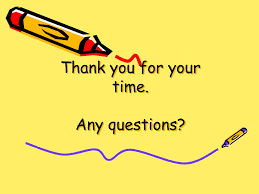
\includegraphics[width=1\linewidth,height=0.79\textheight,keepaspectratio]{thankyou.png}}{[Placeholder: thankyou.png]}
    
    \begin{flushright}
        \tiny\textbf{Email: omar.wasfy@alexu.edu.eg}
    \end{flushright}
    \vfill
\end{frame}

\end{document}